% ****************************************************************************************
% ************************      REPORTE DE BASE DE DATOS     *****************************
% ****************************************************************************************

%  =======================================================
% =======         HEADER FOR DOCUMENT        ============
% =======================================================
    % *********   DOCUMENT ITSELF   **************
    \documentclass[12pt, fleqn]{article}                             %Type of docuemtn and size of font and left eq
    \usepackage[margin=1.2in]{geometry}                             %Margins and Geometry pacakge
    \usepackage{ifthen}                                             %Allow simple programming
    \usepackage{hyperref}                                           %Create MetaData for a PDF and LINKS!
    \hypersetup{pageanchor=false}                                   %Solve 'double page 1' warnings in build
    \setlength{\parindent}{0pt}                                     %Eliminate ugly indentation
    \author{Oscar Andrés Rosas}                                     %Who I am

    % *********   LANGUAJE AND UFT-8   *********
    \usepackage[spanish]{babel}                                     %Please use spanish
    \usepackage[utf8]{inputenc}                                     %Please use spanish - UFT
    \usepackage[T1]{fontenc}                                        %Please use spanish
    \usepackage{textcmds}                                           %Allow us to use quoutes
    \usepackage{changepage}                                         %Allow us to use identate paragraphs
    \usepackage{lipsum}                                             %Allow to put dummy text

    % *********   MATH AND HIS STYLE  *********
    \usepackage{ntheorem, amsmath, amssymb, amsfonts}               %All fucking math, I want all!
    \usepackage{mathrsfs, mathtools, empheq}                        %All fucking math, I want all!
    \usepackage{centernot}                                          %Allow me to negate a symbol
    \decimalpoint                                                   %Use decimal point

    % *********   GRAPHICS AND IMAGES *********
    \usepackage{graphicx}                                           %Allow to create graphics
    \usepackage{wrapfig}                                            %Allow to create images
    \graphicspath{ {Graphics/} }                                    %Where are the images :D

    % *********   LISTS AND TABLES ***********
    \usepackage{listings}                                           %We will be using code here
    \usepackage[inline]{enumitem}                                   %We will need to enumarate
    \usepackage{tasks}                                              %Horizontal lists
    \usepackage{longtable}                                          %Lets make tables awesome
    \usepackage{booktabs}                                           %Lets make tables awesome
    \usepackage{tabularx}                                           %Lets make tables awesome
    \usepackage{multirow}                                           %Lets make tables awesome
    \usepackage{multicol}                                           %Create multicolumns

    % *********   HEADERS AND FOOTERS ********
    \usepackage{fancyhdr}                                           %Lets make awesome headers/footers
    \pagestyle{fancy}                                               %Lets make awesome headers/footers
    \setlength{\headheight}{16pt}                                   %Top line
    \setlength{\parskip}{0.5em}                                     %Top line
    \renewcommand{\footrulewidth}{0.5pt}                            %Bottom line

    \lhead{                                                         %Left Header
        \hyperlink{section.\arabic{section}}                        %Make a link to the current chapter
        {\normalsize{\textsc{\nouppercase{\leftmark}}}}             %And fot it put the name
    }

    \rhead{                                                         %Right Header
        \hyperlink{section.\arabic{section}.\arabic{subsection}}    %Make a link to the current chapter
            {\footnotesize{\textsc{\nouppercase{\rightmark}}}}      %And fot it put the name
    }

    \rfoot{\textsc{\small{Practica 1 y 2}}}                          %This will always be a footer  

    \fancyfoot[L]{                                                  %Algoritm for a changing footer
        \ifthenelse{\isodd{\value{page}}}                           %IF ODD PAGE:
            {\href{https://compilandoconocimiento.com/yo/}          %DO THIS:
                {\footnotesize                                      %Send the page
                    {\textsc{Oscar Andrés Rosas}}}}                 %Send the page
            {\href{https://compilandoconocimiento.com}              %ELSE DO THIS: 
                {\footnotesize                                      %Send the author
                    {\textsc{Compilando Conocimiento}}}}            %Send the author
    }
    
    
    
  
% ========================================
% ===========   COMMANDS    ==============
% ========================================

    % =====  GENERAL TEXT  ==========
    \newcommand \Quote {\qq}                                        %Use: \Quote to use quotes
    \newcommand \Over {\overline}                                   %Use: \Bar to use just for short
    \newcommand \ForceNewLine {$\Space$\\}                          %Use it in theorems for example
    
    \newenvironment{Indentation}[1][0.75em]                         %Use: \begin{Inde...}[Num]...\end{Inde...}
    {\begin{adjustwidth}{#1}{}}                                     %If you dont put nothing i will use 0.75 em
    {\end{adjustwidth}}                                             %This indentate a paragraph
    \newenvironment{SmallIndentation}[1][0.75em]                    %Use: The same that we upper one, just 
    {\begin{adjustwidth}{#1}{}\begin{footnotesize}}                 %footnotesize size of letter by default
    {\end{footnotesize}\end{adjustwidth}}                           %that's it


    % =====  GENERAL MATH  ==========
    \DeclareMathOperator \Space {\quad}                             %Use: \Space for a cool mega space
    \DeclareMathOperator \MiniSpace {\;}                            %Use: \Space for a cool mini space
    \newcommand \Such {\MiniSpace|\MiniSpace}                       %Use: \Such like in sets
    \newcommand \Also {\MiniSpace \text{y} \MiniSpace}              %Use: \Also so it's look cool
    \newcommand \Remember[1]{\Space\text{\scriptsize{#1}}}          %Use: \Remember so it's look cool

    \newtheorem{Theorem}{Teorema}[section]                          %Use: \begin{Theorem}[Name]\label{Nombre}...
    \newtheorem{Corollary}{Colorario}[Theorem]                      %Use: \begin{Corollary}[Name]\label{Nombre}...
    \newtheorem{Lemma}[Theorem]{Lemma}                              %Use: \begin{Lemma}[Name]\label{Nombre}...
    \newtheorem{Definition}{Definición}[section]                    %Use: \begin{Definition}[Name]\label{Nombre}...

    \newcommand{\Set}[1]{\left\{ \MiniSpace #1 \MiniSpace \right\}} %Use: \Set {Info}
    \newcommand{\Brackets}[1]{\left[ #1 \right]}                    %Use: \Brackets {Info} 
    \newcommand{\Wrap}[1]{\left( #1 \right)}                        %Use: \Wrap {Info} 
    \newcommand{\pfrac}[2]{\Wrap{\dfrac{#1}{#2}}}                   %Use: Put fractions in parentesis

    \newenvironment{MultiLineEquation}[1]                           %Use: To create MultiLine equations
        {\begin{equation}\begin{alignedat}{#1}}                     %Use: \begin{Multi..}{Num. de Columnas}
        {\end{alignedat}\end{equation}}                             %And.. that's it!
    \newenvironment{MultiLineEquation*}[1]                          %Use: To create MultiLine equations
        {\begin{equation*}\begin{alignedat}{#1}}                    %Use: \begin{Multi..}{Num. de Columnas}
        {\end{alignedat}\end{equation*}}                            %And.. that's it!


    % =====  LOGIC  ==================
    \DeclareMathOperator \doublearrow {\leftrightarrow}             %Use: \doublearrow for a double arrow
    \newcommand \lequal {\MiniSpace \Leftrightarrow \MiniSpace}     %Use: \lequal for a double arrow
    \newcommand \linfire {\MiniSpace \Rightarrow \MiniSpace}        %Use: \lequal for a double arrow
    \newcommand \longto {\longrightarrow}                           %Use: \longto for a long arrow

    % =====  NUMBER THEORY  ==========
    \DeclareMathOperator \Naturals  {\mathbb{N}}                     %Use: \Naturals por Notation
    \DeclareMathOperator \Primes    {\mathbb{P}}                     %Use: \Naturals por Notation
    \DeclareMathOperator \Integers  {\mathbb{Z}}                     %Use: \Integers por Notation
    \DeclareMathOperator \Racionals {\mathbb{Q}}                     %Use: \Racionals por Notation
    \DeclareMathOperator \Reals     {\mathbb{R}}                     %Use: \Reals por Notation
    \DeclareMathOperator \Complexs  {\mathbb{C}}                     %Use: \Complex por Notation

    % === LINEAL ALGEBRA & VECTORS ===
    \DeclareMathOperator \LinealTransformation {\mathcal{T}}        %Use: \LinealTransformation for a cool T
    \newcommand{\Mag}[1]{\left| #1 \right|}                         %Use: \Mag {Info} 

    \newcommand{\pVector}[1]{                                       %Use: \pVector {Matrix Notation} use parentesis
        \ensuremath{\begin{pmatrix}#1\end{pmatrix}}                 %Example: \pVector{a\\b\\c} or \pVector{a&b&c} 
    }
    \newcommand{\lVector}[1]{                                       %Use: \lVector {Matrix Notation} use a abs 
        \ensuremath{\begin{vmatrix}#1\end{vmatrix}}                 %Example: \lVector{a\\b\\c} or \lVector{a&b&c} 
    }
    \newcommand{\bVector}[1]{                                       %Use: \bVector {Matrix Notation} use a brackets 
        \ensuremath{\begin{bmatrix}#1\end{bmatrix}}                 %Example: \bVector{a\\b\\c} or \bVector{a&b&c} 
    }
    \newcommand{\Vector}[1]{                                        %Use: \Vector {Matrix Notation} no parentesis
        \ensuremath{\begin{matrix}#1\end{matrix}}                   %Example: \Vector{a\\b\\c} or \Vector{a&b&c}
    }

    % MATRIX
    \makeatletter                                                   %Example: \begin{matrix}[cc|c]
    \renewcommand*\env@matrix[1][*\c@MaxMatrixCols c] {             %WTF! IS THIS
        \hskip -\arraycolsep                                        %WTF! IS THIS
        \let\@ifnextchar\new@ifnextchar                             %WTF! IS THIS
        \array{#1}                                                  %WTF! IS THIS
    }                                                               %WTF! IS THIS
    \makeatother                                                    %WTF! IS THIS

    % TRIGONOMETRIC FUNCTIONS
    \newcommand{\Cos}[1]{\cos\Wrap{#1}}                             %Simple wrappers
    \newcommand{\Sin}[1]{\sin\Wrap{#1}}                             %Simple wrappers

    % === COMPLEX ANALYSIS ===
    \newcommand \Cis[1]  {\Cos{#1} + i \Sin{#1}}                    %Use: \Cis for cos(x) + i sin(x)
    \newcommand \pCis[1] {\Wrap{\Cis{#1}}}                          %Use: \pCis for the same ut parantesis
    \newcommand \bCis[1] {\Brackets{\Cis{#1}}}                      %Use: \bCis for the same to Brackets

    % === CALCULUS ===
    \newcommand \Partial[2] {\dfrac{\partial #1}{\partial #2}}      %Use: \Partial for simple use

    % =====  GENERAL COLOR  =========
    \definecolor{IndigoMD}{HTML}{3F51B5}                            %Use: Color :D
    \definecolor{DeepPurpleMD}{HTML}{673AB7}                        %Use: Color :D
    \definecolor{TealMD}{HTML}{009688}                              %Use: Color :D        
    \definecolor{BlueGrey800MD}{HTML}{37474F}                       %Use: Color :D
    \definecolor{BlueGrey100MD}{HTML}{CFD8DC}                       %Use: Color :D
    \definecolor{IndigoMD}{HTML}{3F51B5}                            %Use: Color :D
    \definecolor{Green100MD}{HTML}{DCEDC8}                          %Use: Color :D

    \newenvironment{ColorText}[1]{                                  %Use: \begin{ColorText}
        \leavevmode\color{#1}\ignorespaces}                         %That's is!


    % =====  CODE EDITOR =========
    \lstdefinestyle{CompilandoStyle} {                              %This is Code Style
        backgroundcolor=\color{BlueGrey800MD},                      %Background Color  
        basicstyle=\tiny\color{white},                              %Font color
        commentstyle=\color{BlueGrey100MD},                         %Comment color
        stringstyle=\color{TealMD},                                 %String color
        keywordstyle=\color{Green100MD},                            %keywords color
        numberstyle=\tiny\color{TealMD},                            %Size of a number
        frame=shadowbox,                                            %Adds a frame around the code
        breakatwhitespace=true,                                     %Style                       
        breaklines=true,                                            %Style                   
        keepspaces=true,                                            %Style                   
        numbers=left,                                               %Style                   
        numbersep=10pt,                                             %Style 
        xleftmargin=\parindent,                                     %Style 
        tabsize=4                                                   %Style 
    }
 
    \lstset{style=CompilandoStyle}                                  %Use this style



% =====================================================
% ============        COVER PAGE       ================
% =====================================================
\begin{document}
\begin{titlepage}

    \center
    % ============ UNIVERSITY NAME AND DATA =========
    \textsc{\Large ESCOM - IPN}\\[0.5cm] 
    \textsc{\large Bases de Datos 2CM12}\\[1.5cm]

    % ============ NAME OF THE DOCUMENT  ============
    \rule{\linewidth}{0.5mm} \\[1.0cm]
        { \huge \bfseries Querys.... Muchos Querys}\\[1.0cm] 
    \rule{\linewidth}{0.5mm} \\[2.0cm]
     
    % ============  MY INFORMATION  =================
    \begin{minipage}{0.4\textwidth}
        \begin{flushleft} \large
            \textbf{\textsc{Alumno:}}\\
            Rosas Hernandez Oscar Andres
        \end{flushleft}
    \end{minipage}
    ~
    \begin{minipage}{0.4\textwidth}
        \begin{flushright} \large
            \textbf{\textsc{Profesor: }}\\
            Euler Hernandez Contreras
        \end{flushright}
    \end{minipage}\\[3,5cm]

    % ====== SEMI TITLE ==========
    {\LARGE Reporte 3 y Reporte 4}\\[4cm] 
    
    
    \vfill

\end{titlepage}









% ===============================================================================
% ===================        QUERIES EN SQL                ======================
% ===============================================================================
\section{Queries en SQL}

    % ========================================
    % =========   SELECT FROM    =============
    % ========================================
    \subsection{SELECT FROM}

        Empecemos por la sentencia más básica para un Query en SQL:

        \begin{lstlisting}[language=SQL, gobble=12]
            SELECT FielName FROM TableName;
        \end{lstlisting}

        Ahora empecemos por aquí:
        \subsection{Distint vs All}
        \begin{itemize}
            \item Distint (Default):
                Esta solo muestra solo los atributos diferentes

                \begin{lstlisting}[language=SQL, gobble=20]
                    SELECT DISTINT FielName FROM TableName;
                \end{lstlisting}
            \item All:
                Esta muestra todos los atributos, incluso duplicados
                \begin{lstlisting}[language=SQL, gobble=20]
                    SELECT ALL FielName FROM TableName;
                \end{lstlisting}
        \end{itemize}



    % ========================================
    % =========   COUNT , AVE, SUM  ==========
    % ========================================
    \subsection{Funciones de Agregación}

        Las funciones de agregación son funciones que toman una colección
        como entrada y regresan un simple valor. SQL ofrece estas 5 funciones
        por default:

        \begin{itemize}
            \item \Quote{AVG()}: Promedio
            \item \Quote{MIN()}: Minimo
            \item \Quote{MAX()}: Máximo
            \item \Quote{COUNT()}: Cuenta la cantidad 
            \item \Quote{SUM()}: Suma todo el resultado
        \end{itemize}





    % ========================================
    % ============     WHERE   ===============
    % ========================================
    \clearpage
    \subsection{WHERE}

        Esta nos permite seleccionar solo las filas en el resultado del quey
        que satisface nuestros criterios.

        \begin{lstlisting}[language=SQL, gobble=12]
            SELECT FielName FROM TableName
                WHERE
                    (TableName.Thing1 < Something) AND
                    (TableName.Thing2 = "Some Strings");
        \end{lstlisting}

        Tenemos a nuestra dispoción los siguientes comparadores:
        \begin{itemize}
            \item Lógicos: AND, OR, NOT
            \item Aritmeticos: <, >, <=, >=, =, <>
        \end{itemize}



    % ========================================
    % ============   STRINGS   ===============
    % ========================================
    \subsection{Comparación de Strings}
        
        Podemos comparar strings gracias a lo que conocemos como comodínes usando
        el comando \Quote{LIKE}
        \begin{itemize}
            \item \Quote{\%}: Que sirve como comodín para cualquier cantidad de caracteres 
            \item \Quote{\_}: Que sirve como comodín para un caracter 
        \end{itemize}


    % ========================================
    % ========   ORDEN DE TUPLAS   ===========
    % ========================================
    \subsection{Orden de las Tuplas}

        Podemos controlar el orden en que se nos retornan las tuplas del query que estamos
        haciendo muy facilmente con la instructiva ORDER BY.

        Por default se usa la opción \Quote{ASC} que las ordena de manera ascendente
        mientras que \Quote{DESC} la ordena de manera descendente.

        Por default esta se coloca la última línea de manera implicita:
        \begin{lstlisting}[language=SQL, gobble=12]
            SELECT DISTINT FielName1, FielName2, FielName3 FROM TableName
                ORDER BY FielName1 ASC, FielName2 ASC, FielName3 ASC;
        \end{lstlisting}

        También podemos simplemente poner el número en que las pusimos para 
        indicar el orden:

        \begin{lstlisting}[language=SQL, gobble=12]
            SELECT DISTINT FielName1, FielName2, FielName3 FROM TableName
                ORDER BY 1,2, 3;
        \end{lstlisting}




% ===============================================================================
% ===================             PRACTICA 3               ======================
% ===============================================================================
\clearpage
\section{Parte Practica: Practica 3}

    Veamor por pasos que es lo que hicimos:

    \begin{itemize}

        \item
            \textbf{Mostramos: Nombre de asociado y sucursal donde esta asignado}
            \lstinputlisting[language=SQL, linerange={7-12}]{Practica3.sql}

        \item
            \textbf{Mostramos: Nombre de clubes existentes en DF}
            \lstinputlisting[language=SQL, linerange={15-19}]{Practica3.sql}

        \item
            \textbf{Mostramos: Nombre de clubes existentes en NuevoLeon}
            \lstinputlisting[language=SQL, linerange={23-27}]{Practica3.sql}

        \item
            \textbf{Mostramos: Nombre de clubes existentes en Tamaulipas}
            \lstinputlisting[language=SQL, linerange={31-35}]{Practica3.sql}

        \item
            \textbf{Mostramos: Nombre del socio y la tarjeta asignada}
            \lstinputlisting[language=SQL, linerange={39-43}]{Practica3.sql}


        \item
            \textbf{Mostramos: Nombre del socio y la tarjeta asignada y que se apellida Hernandez}
            \lstinputlisting[language=SQL, linerange={47-51}]{Practica3.sql}

        \item
            \textbf{Mostramos: Nombre de los departamentos de una sucursal determinada}
            \lstinputlisting[language=SQL, linerange={55-59}]{Practica3.sql}

        \item
            \textbf{Mostramos: El credito que tienen los socios que se apellidan como Garcia}
            \lstinputlisting[language=SQL, linerange={63-67}]{Practica3.sql}

        \item
            \textbf{Mostramos: Cuantos socios tienen la tarjeta DECORE}
            \lstinputlisting[language=SQL, linerange={71-74}]{Practica3.sql}

        \item
            \textbf{Mostramos: Como se llaman los socios de la consulta anterior}
            \lstinputlisting[language=SQL, linerange={78-81}]{Practica3.sql}

        \item
            \textbf{Mostramos: Cuantos asociados tienen como apellido paterno Perez}
            \lstinputlisting[language=SQL, linerange={85-88}]{Practica3.sql}

        \item
            \textbf{Mostramos: Como se llaman los asociados de la consulta anterior}
            \lstinputlisting[language=SQL, linerange={91-94}]{Practica3.sql}




        \item
            \textbf{Mostramos: Proyectar las sucursales donde estan asignados
            los asociados donde proyectar es ordenar la salida y eliminar campos}
            \lstinputlisting[language=SQL, linerange={98-102}]{Practica3.sql}

        \item
            \textbf{Mostramos: Mostrar el nombre de las siguientes sucursales y
            sus asociados con CP 78045, 89360, 25279.}
            \lstinputlisting[language=SQL, linerange={106-115}]{Practica3.sql}

        \clearpage

        \item
            \textbf{Mostramos: Como se llaman los asociados que tienen Metepec como sucursal}
            \lstinputlisting[language=SQL, linerange={119-124}]{Practica3.sql}

        \item
            \textbf{Mostramos: Que telefeno tienen los socios que tiene la 
            tarjeta Pagos Fijos y mostrar la sucursal donde de se encuentran
            dados de alta.}
            \lstinputlisting[language=SQL, linerange={128-137}]{Practica3.sql}

        \item
            \textbf{Mostramos: Mostrar los departamentos que tiene la sucursal Tijuana}
            \lstinputlisting[language=SQL, linerange={141-148}]{Practica3.sql}

        \item
            \textbf{Mostramos: Como se llaman las sucursales que tienen el departamento de pisos}
            \lstinputlisting[language=SQL, linerange={152-159}]{Practica3.sql}

    \end{itemize}


    % ================================================================
    % ===================       EVIDENCIAS           =================
    % ================================================================
    \clearpage
    \subsection{Evidencias}

        \begin{figure}[ht!]
            \centering
            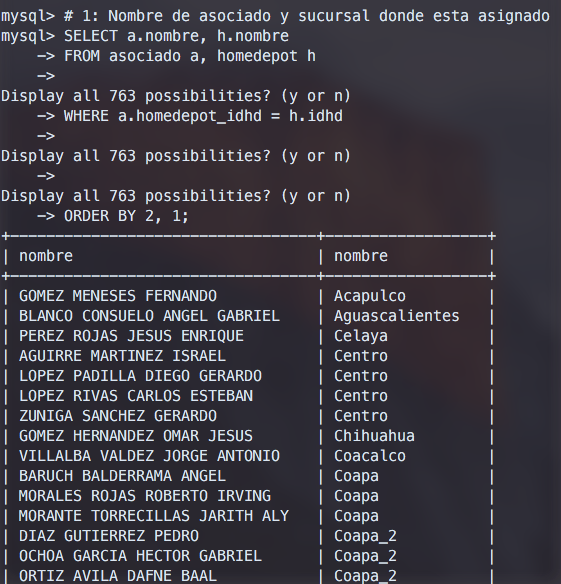
\includegraphics[width=0.35\textwidth]{BD3Reporte0}
            \caption{Nombre de asociado y sucursal donde esta asignado}
        \end{figure}

        \begin{figure}[ht!]
            \centering
            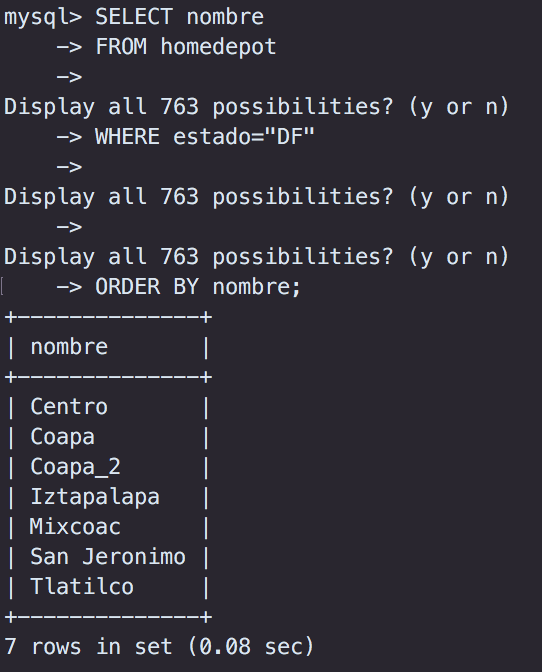
\includegraphics[width=0.35\textwidth]{BD3Reporte1}
            \caption{Nombre de clubes existentes en DF}
        \end{figure}


        \begin{figure}[ht!]
            \centering
            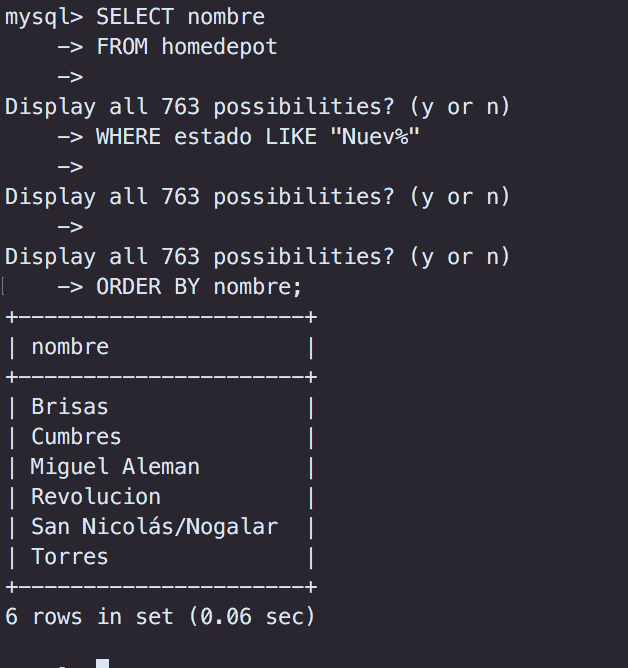
\includegraphics[width=0.35\textwidth]{BD3Reporte2}
            \caption{Nombre de clubes existentes en NuevoLeon}
        \end{figure}

        \begin{figure}[ht!]
            \centering
            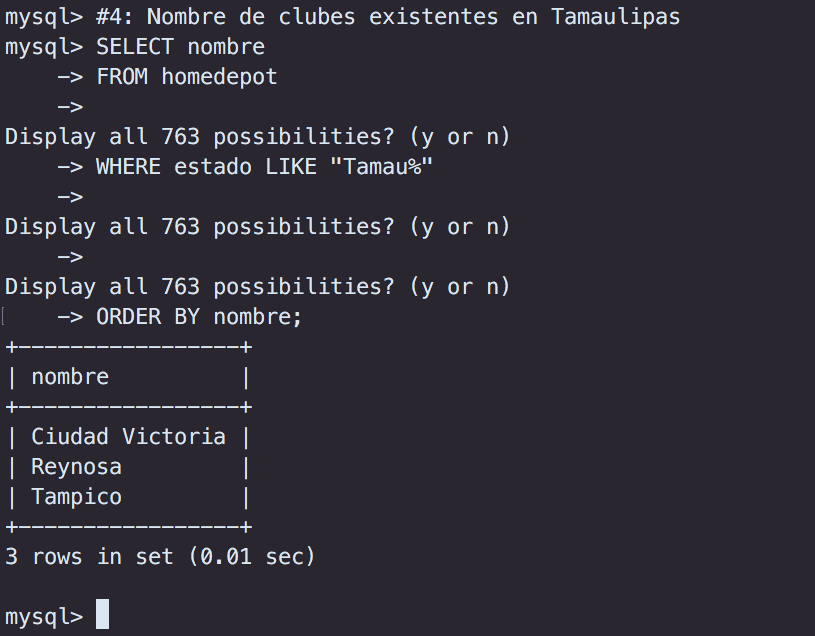
\includegraphics[width=0.35\textwidth]{BD3Reporte3}
            \caption{Nombre de clubes existentes en Tamaulipas}
        \end{figure}

        \begin{figure}[ht!]
            \centering
            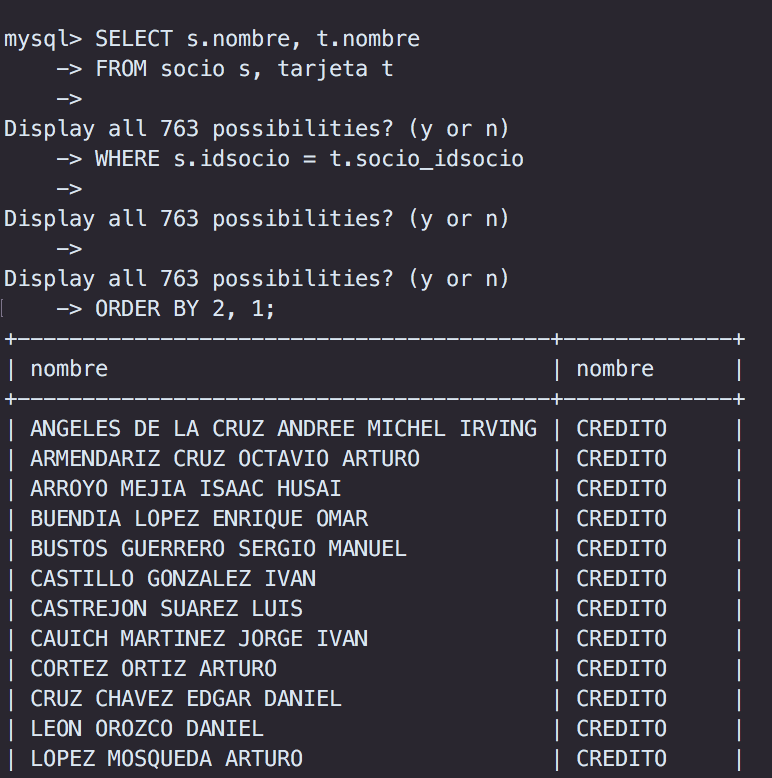
\includegraphics[width=0.35\textwidth]{BD3Reporte4}
            \caption{Nombre del socio y la tarjeta asignada}
        \end{figure}

        \begin{figure}[ht!]
            \centering
            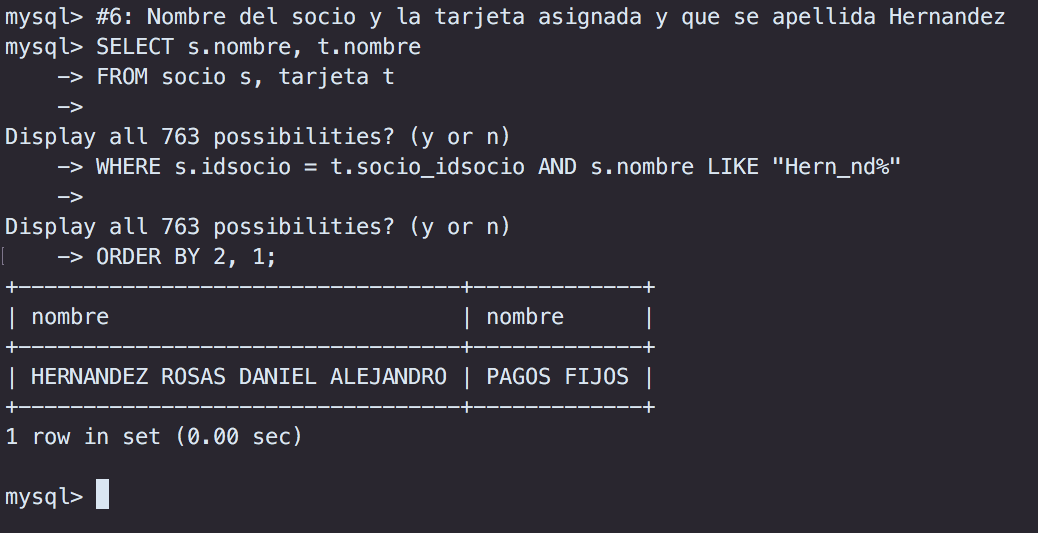
\includegraphics[width=0.45\textwidth]{BD3Reporte5}
            \caption{Nombre del socio y la tarjeta asignada y que se apellida Hernandez}
        \end{figure}

        \begin{figure}[ht!]
            \centering
            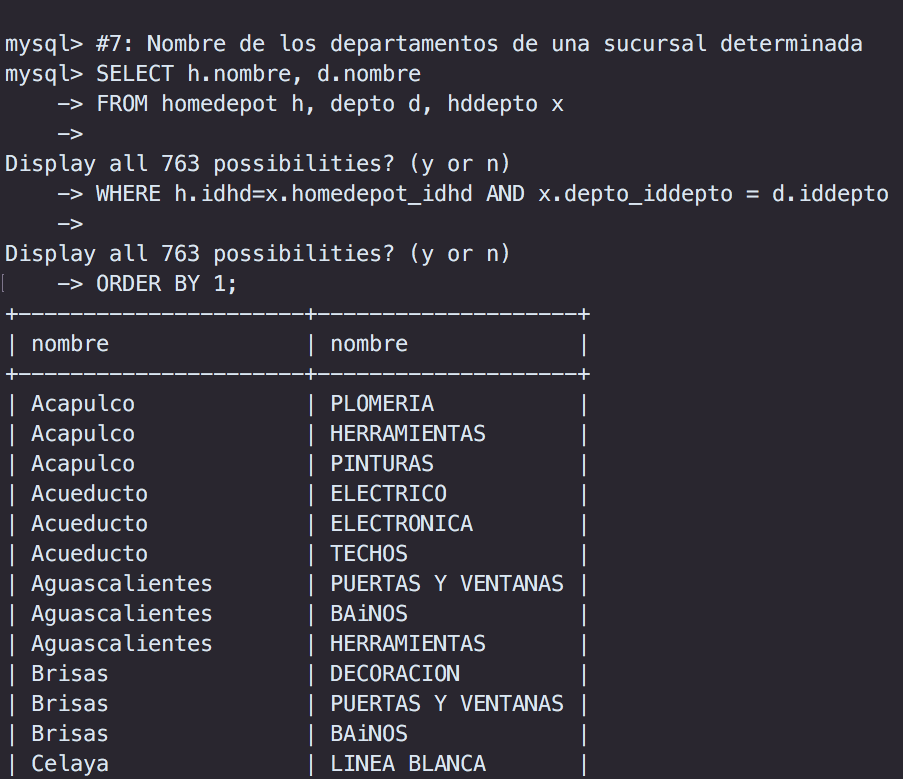
\includegraphics[width=0.45\textwidth]{BD3Reporte6}
            \caption{Nombre de los departamentos de una sucursal determinada}
        \end{figure}


        \begin{figure}[ht!]
            \centering
            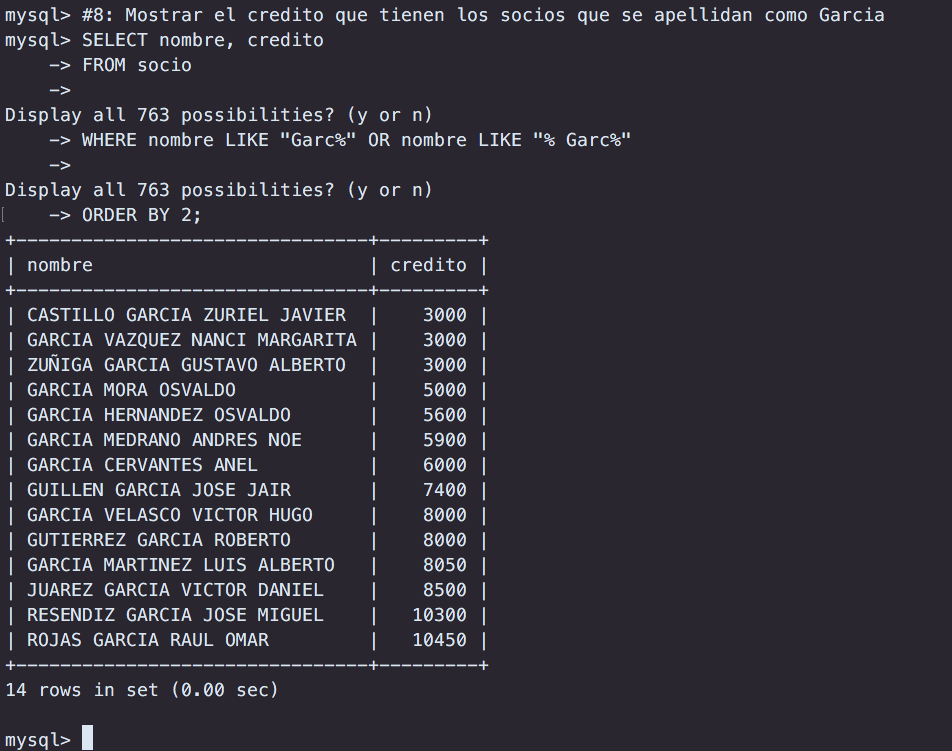
\includegraphics[width=0.45\textwidth]{BD3Reporte7}
            \caption{Mostrar el credito que tienen los socios que se apellidan como Garcia}
        \end{figure}

        \begin{figure}[ht!]
            \centering
            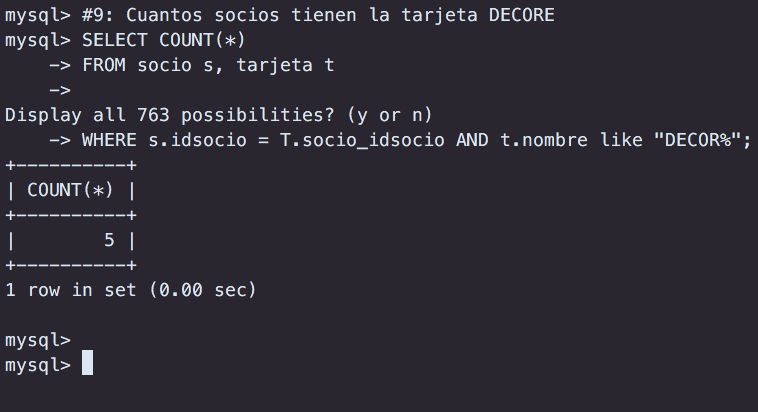
\includegraphics[width=0.45\textwidth]{BD3Reporte8}
            \caption{Cuantos socios tienen la tarjeta DECORE}
        \end{figure}

        \begin{figure}[ht!]
            \centering
            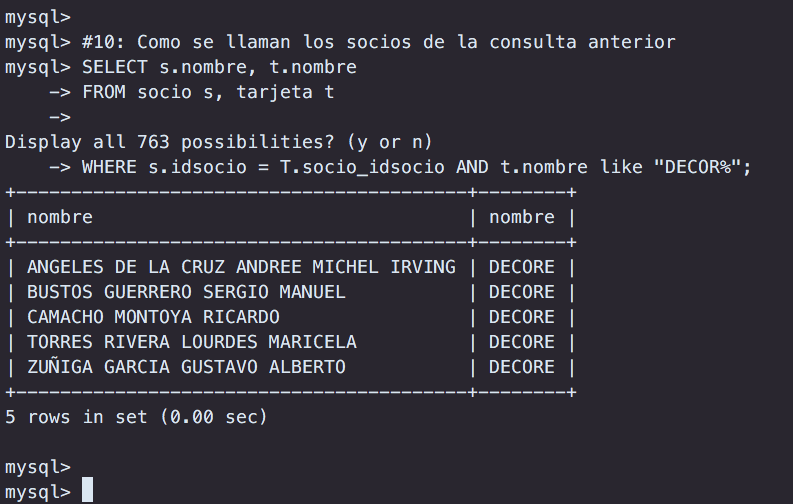
\includegraphics[width=0.45\textwidth]{BD3Reporte9}
            \caption{Como se llaman los socios de la consulta anterior}
        \end{figure}

        \begin{figure}[ht!]
            \centering
            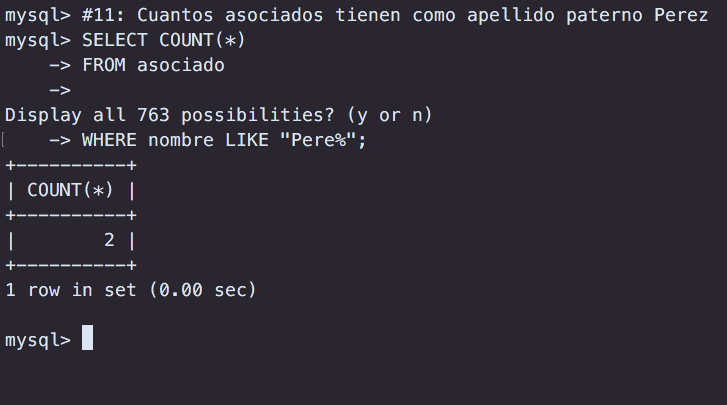
\includegraphics[width=0.45\textwidth]{BD3Reporte10}
            \caption{Cuantos asociados tienen como apellido paterno Perez}
        \end{figure}

        \begin{figure}[ht!]
            \centering
            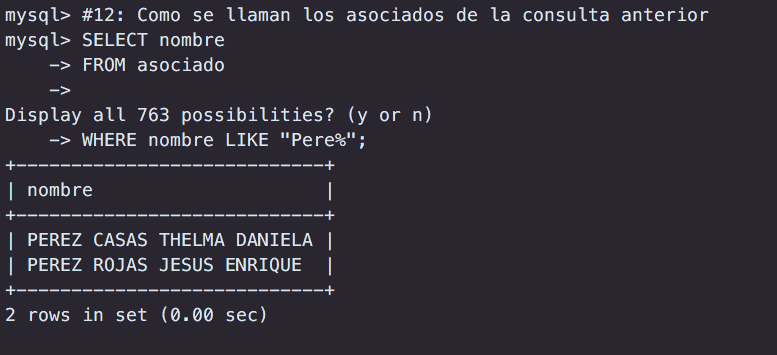
\includegraphics[width=0.45\textwidth]{BD3Reporte11}
            \caption{Como se llaman los asociados de la consulta anterior}
        \end{figure}

        \begin{figure}[ht!]
            \centering
            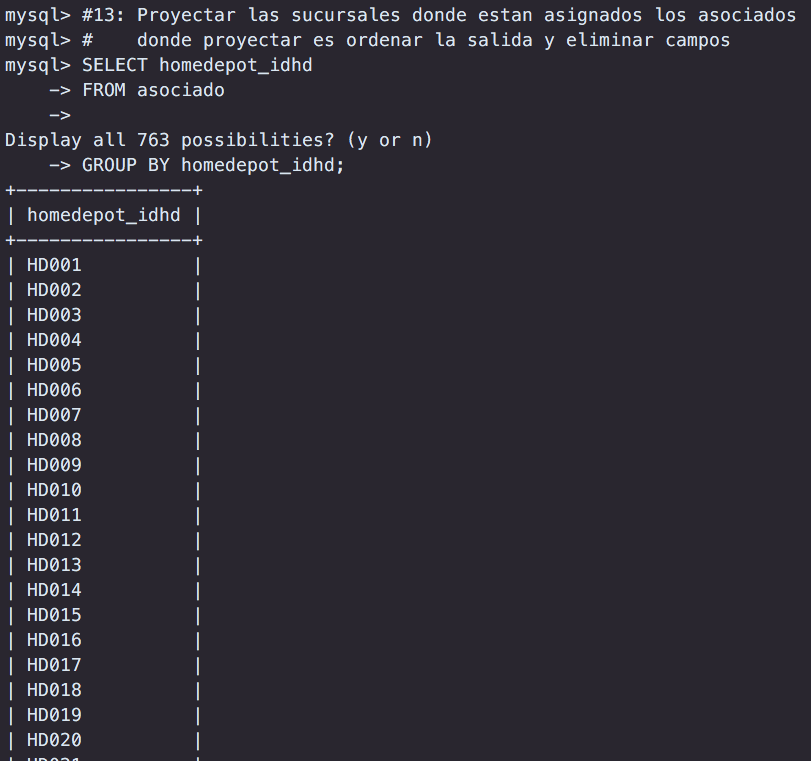
\includegraphics[width=0.45\textwidth]{BD3Reporte12}
            \caption{Proyectar las sucursales donde estan asignados los asociados
            donde proyectar es ordenar la salida y eliminar campos}
        \end{figure}

        \begin{figure}[ht!]
            \centering
            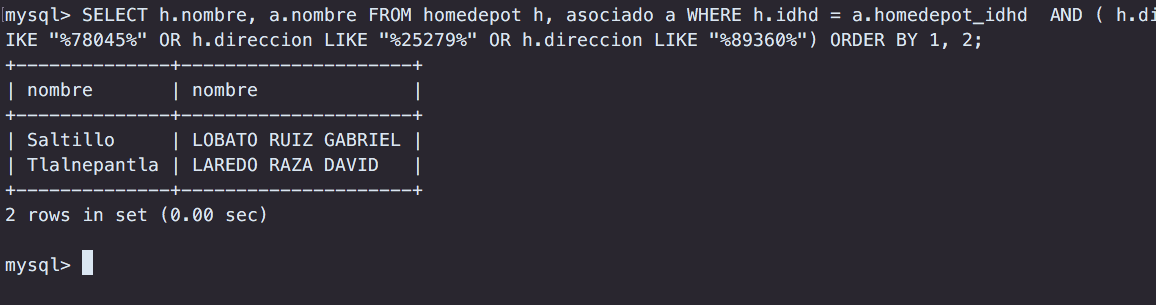
\includegraphics[width=0.45\textwidth]{BD3Reporte13}
            \caption{Mostrar el nombre de las siguientes sucursales y sus asociados con CP 78045, 89360, 25279.}
        \end{figure}


        \begin{figure}[ht!]
            \centering
            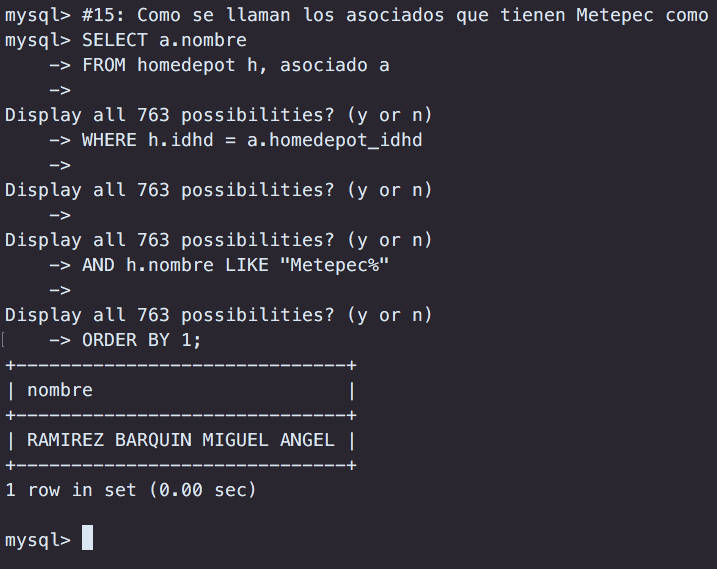
\includegraphics[width=0.45\textwidth]{BD3Reporte14}
            \caption{Como se llaman los asociados que tienen Metepec como sucursal}
        \end{figure}

        \begin{figure}[ht!]
            \centering
            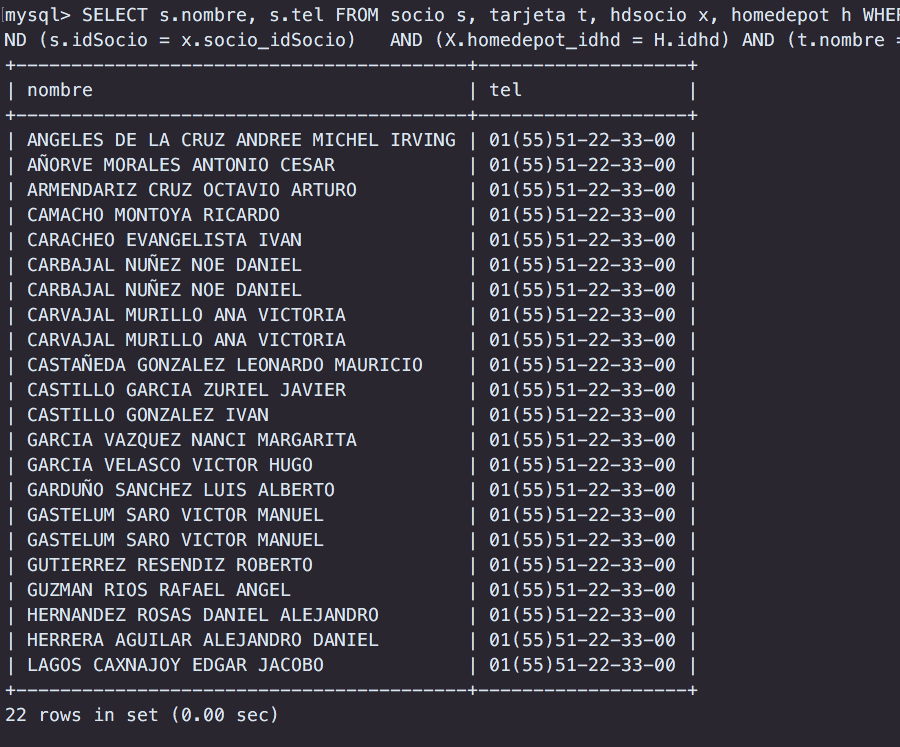
\includegraphics[width=0.45\textwidth]{BD3Reporte15}
            \caption{Que telefeno tienen los socios que tiene la tarjeta Pagos Fijos y mostrar la sucursal donde de se encuentran dados de alta}
        \end{figure}

        \begin{figure}[ht!]
            \centering
            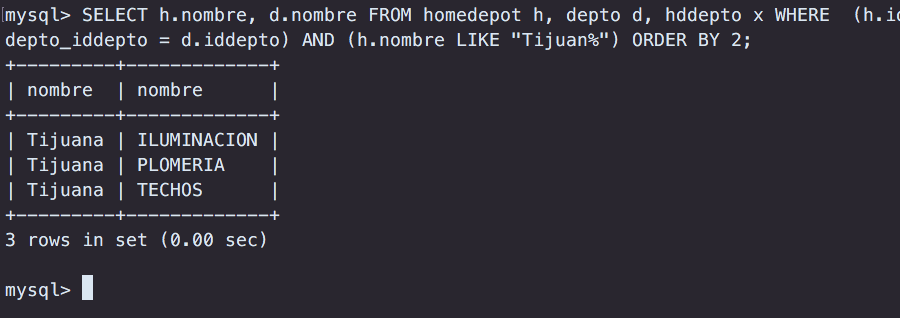
\includegraphics[width=0.45\textwidth]{BD3Reporte16}
            \caption{Mostrar los departamentos que tiene la sucursal Tijuana}
        \end{figure}

        \begin{figure}[ht!]
            \centering
            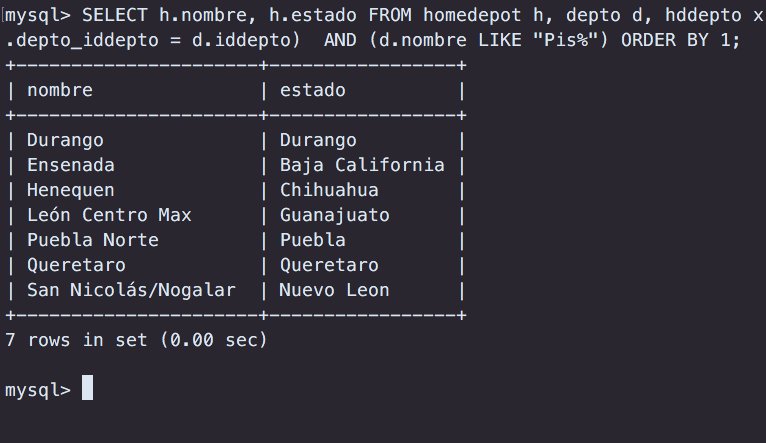
\includegraphics[width=0.45\textwidth]{BD3Reporte17}
            \caption{Como se llaman las sucursales que tienen el departamento de pisos}
        \end{figure}






% ===============================================================================
% ===================             PRACTICA 4               ======================
% ===============================================================================
\clearpage
\section{Parte Practica: Practica 4}

    Veamor por pasos que es lo que hicimos:

    \begin{itemize}

        \item
            \textbf{Conocer el no de tt, de aquellos tts que ha dirigido el Director}
            \lstinputlisting[language=SQL, linerange={6-13}]{Practica4.sql}

        \item
            \textbf{Cuantos tts ha dirigido el tio flavio }
            \lstinputlisting[language=SQL, linerange={17-24}]{Practica4.sql}

        \item
            \textbf{Cual es titulo de los tts de la consulta anterior}
            \lstinputlisting[language=SQL, linerange={28-36}]{Practica4.sql}

        \item
            \textbf{Que no. de tt tienen aquellos tts que se han presentado en el año 2008}
            \lstinputlisting[language=SQL, linerange={40-44}]{Practica4.sql}

        \item
            \textbf{Mostrar el tipo de tt que ha dirigido su profe de bases}
            \lstinputlisting[language=SQL, linerange={48-57}]{Practica4.sql}

        \item
            \textbf{Grado de Garcias}
            \lstinputlisting[language=SQL, linerange={61-68}]{Practica4.sql}

        \item
            \textbf{Profesores de la UNAM}
            \lstinputlisting[language=SQL, linerange={71-75}]{Practica4.sql}

        \item
            \textbf{Mostrar el no. de tt y el tipo, ademas del dictamen de aquellos tts donde la Dra. Lorena Chavarria ha sido sinodal.}
            \lstinputlisting[language=SQL, linerange={79-89}]{Practica4.sql}

        \item
            \textbf{Mostrar el no de tt y la fecha de presentacion de aquellos tts que incluyen la palabra Redes neuronales.}
            \lstinputlisting[language=SQL, linerange={93-98}]{Practica4.sql}

        \item
            \textbf{Mostrar el no de tt y el nombre de los directores que han dirigido tt remediales}
            \lstinputlisting[language=SQL, linerange={102-110}]{Practica4.sql}

        \item
            \textbf{Mostrar la cedula profesional y la institucion de aquellos profesores que
            tienen grado de maestría}
            \lstinputlisting[language=SQL, linerange={114-122}]{Practica4.sql}

        \clearpage

        \item
            \textbf{Mostrar el no de tt, la calificación de los sinodales, donde el revisor ha
            sido la Dra. Fabiola Ocampo}
            \lstinputlisting[language=SQL, linerange={126-135}]{Practica4.sql}


        \item
            \textbf{Mostrar los sinodales que han tenido los siguientes tts: 2000-0209, 06-1-0174}
            \lstinputlisting[language=SQL, linerange={139-144}]{Practica4.sql}

        \item
            \textbf{¿Quién fue el revisor del tt que ha dirigido Idalia Maldonado?}
            \lstinputlisting[language=SQL, linerange={148-156}]{Practica4.sql}

    \end{itemize}


    % ================================================================
    % ===================       EVIDENCIAS           =================
    % ================================================================
    \clearpage
    \subsection{Evidencias}

        \begin{figure}[ht!]
            \centering
            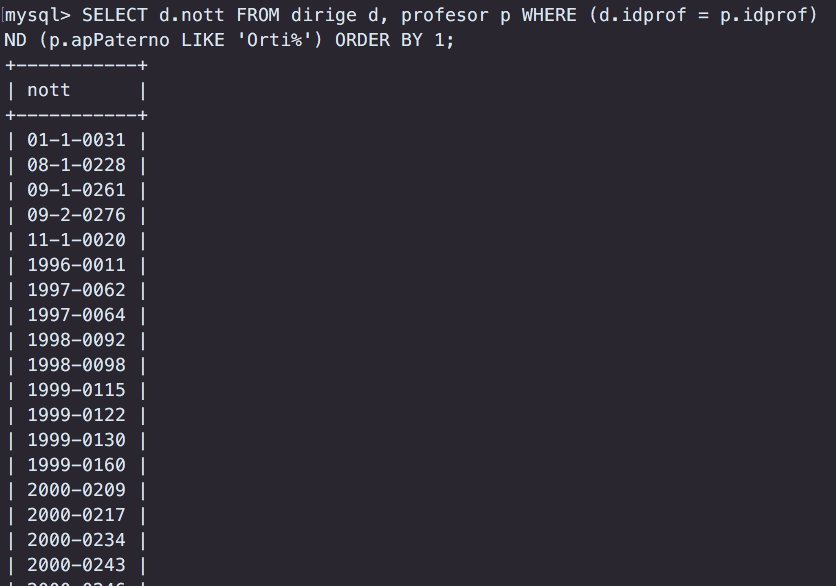
\includegraphics[width=0.35\textwidth]{BD4Reporte1}
            \caption{Conocer el no. de tt, de aquellos tts que ha dirigido el Director}
        \end{figure}

        \begin{figure}[ht!]
            \centering
            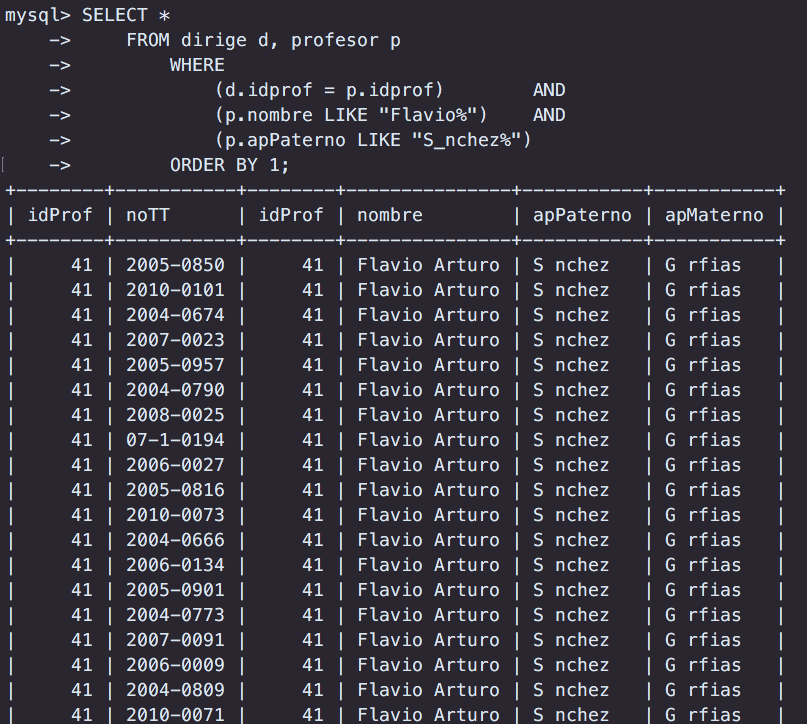
\includegraphics[width=0.35\textwidth]{BD4Reporte2}
            \caption{Cuantos tts ha dirigido el tio flavio}
        \end{figure}


        \begin{figure}[ht!]
            \centering
            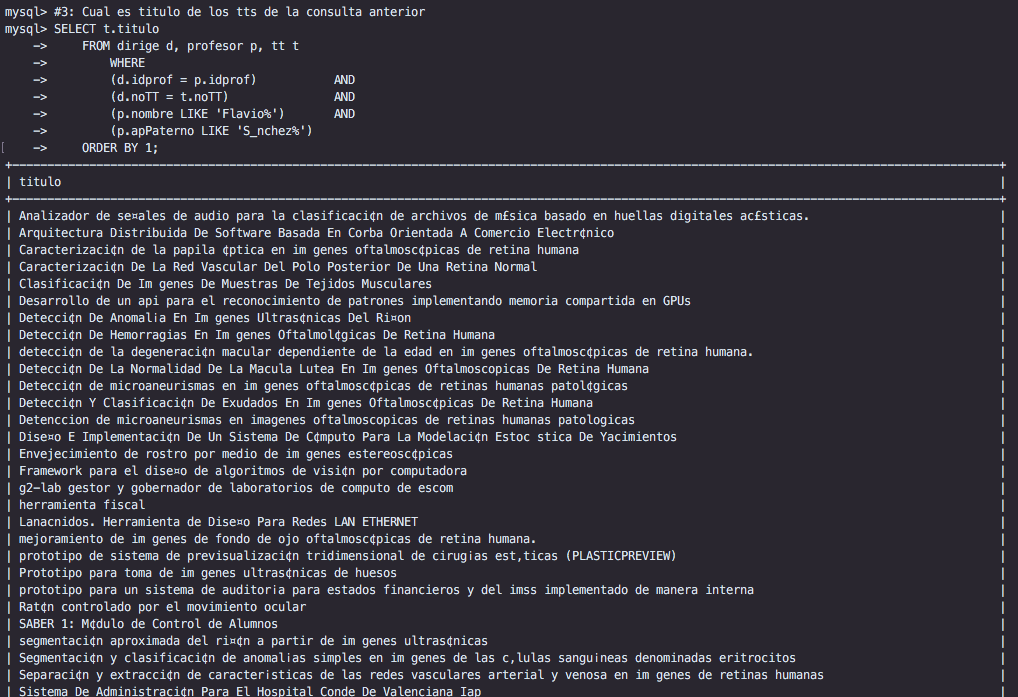
\includegraphics[width=0.35\textwidth]{BD4Reporte3}
            \caption{Cual es titulo de los tts de la consulta anterior}
        \end{figure}

        \begin{figure}[ht!]
            \centering
            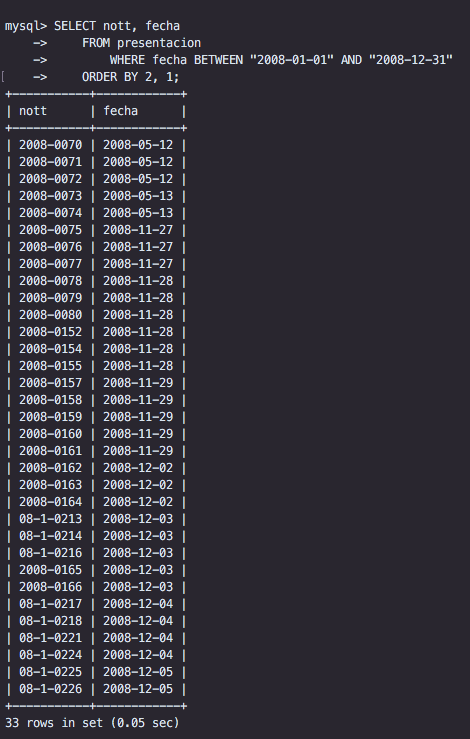
\includegraphics[width=0.35\textwidth]{BD4Reporte4}
            \caption{Que no. de tt tienen aquellos tts que se han presentado en el año 2008}
        \end{figure}

        \begin{figure}[ht!]
            \centering
            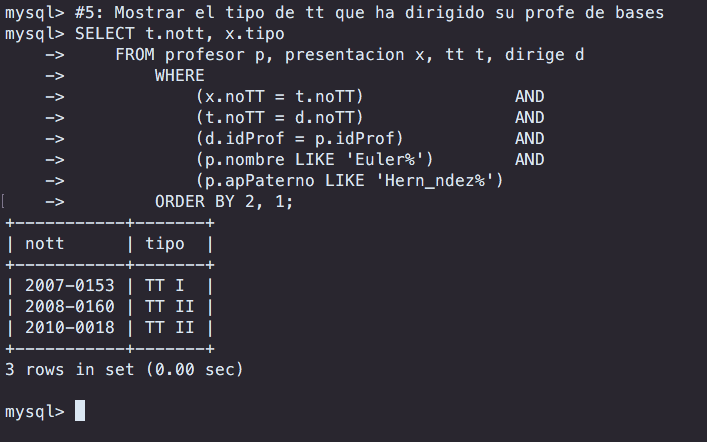
\includegraphics[width=0.35\textwidth]{BD4Reporte5}
            \caption{Mostrar el tipo de tt que ha dirigido su profe de bases}
        \end{figure}


        \begin{figure}[ht!]
            \centering
            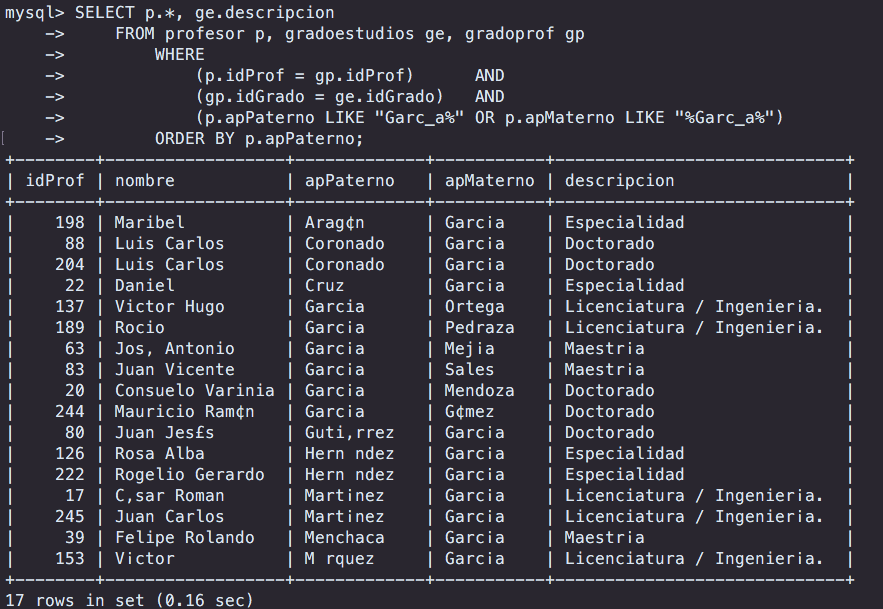
\includegraphics[width=0.45\textwidth]{BD4Reporte6}
            \caption{Grado de Garcias}
        \end{figure}

        \begin{figure}[ht!]
            \centering
            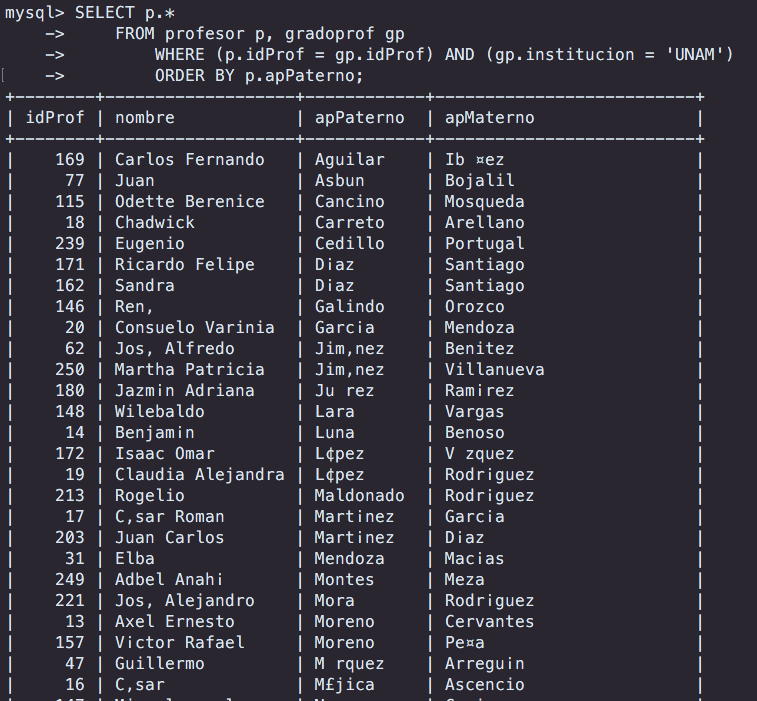
\includegraphics[width=0.45\textwidth]{BD4Reporte7}
            \caption{Profesores de la UNAM}
        \end{figure}


        \begin{figure}[ht!]
            \centering
            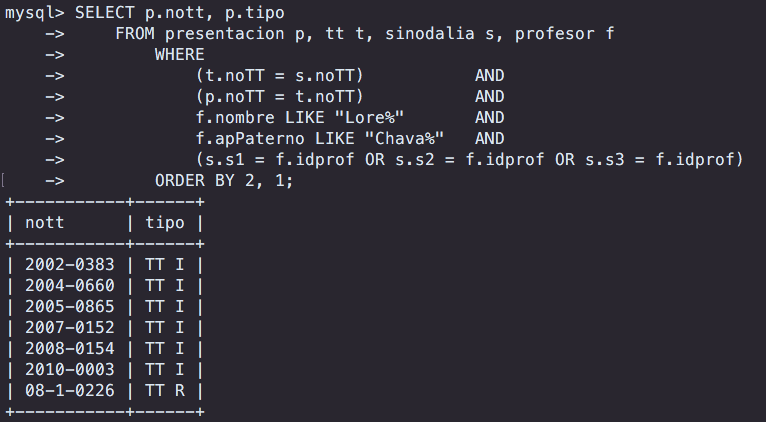
\includegraphics[width=0.45\textwidth]{BD4Reporte8}
            \caption{Mostrar el no. de tt y el tipo, ademas del dictamen de aquellos tts donde
            la Dra. Lorena Chavarria ha sido sinodal.}
        \end{figure}

        \begin{figure}[ht!]
            \centering
            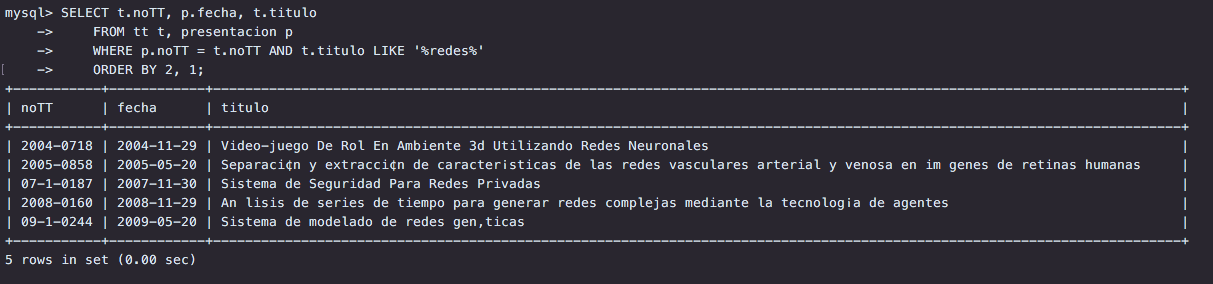
\includegraphics[width=0.45\textwidth]{BD4Reporte9}
            \caption{Mostrar el no de tt y la fecha de presentacion de aquellos tts que
            incluyen la palabra Redes neuronales}
        \end{figure}

        \begin{figure}[ht!]
            \centering
            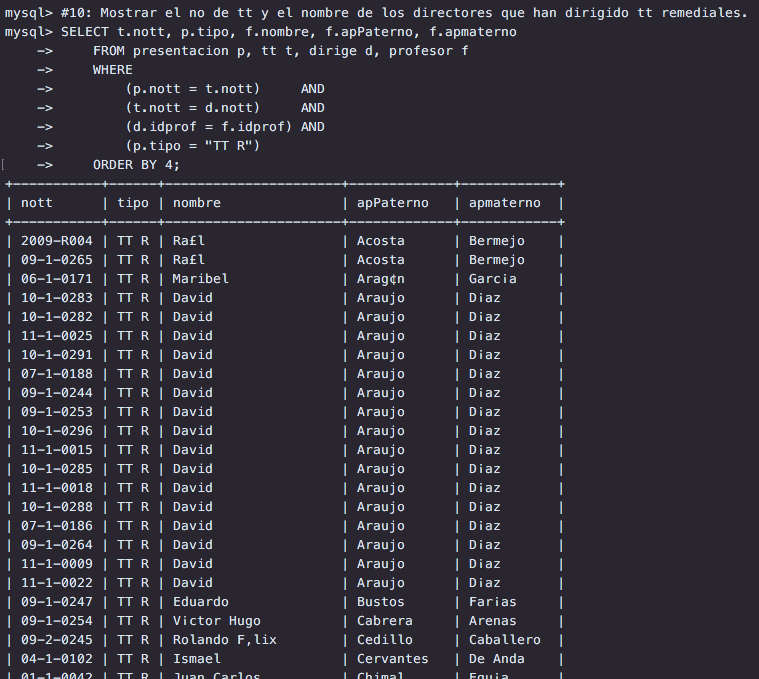
\includegraphics[width=0.45\textwidth]{BD4Reporte10}
            \caption{ostrar el no de tt y el nombre de los directores que han dirigido tt
            remediales}
        \end{figure}

        \begin{figure}[ht!]
            \centering
            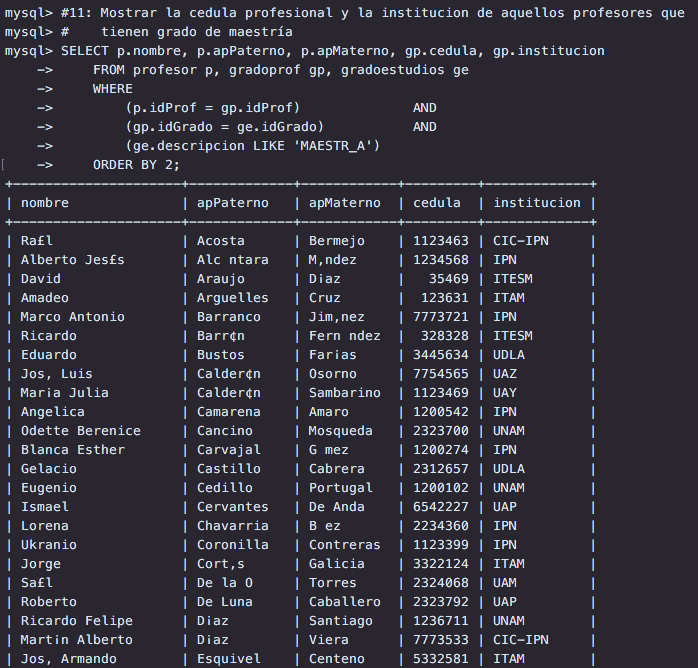
\includegraphics[width=0.45\textwidth]{BD4Reporte11}
            \caption{Mostrar la cedula profesional y la institucion de aquellos profesores que
            tienen grado de maestría}
        \end{figure}

        \begin{figure}[ht!]
            \centering
            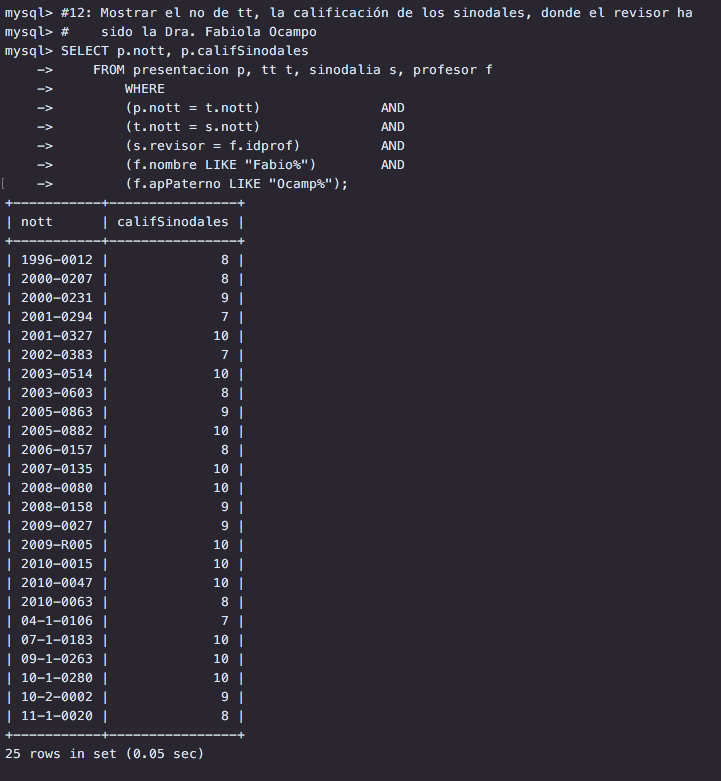
\includegraphics[width=0.45\textwidth]{BD4Reporte12}
            \caption{Mostrar el no de tt, la calificación de los sinodales, donde el revisor
            ha sido la Dra. Fabiola Ocampo}
        \end{figure}

        \begin{figure}[ht!]
            \centering
            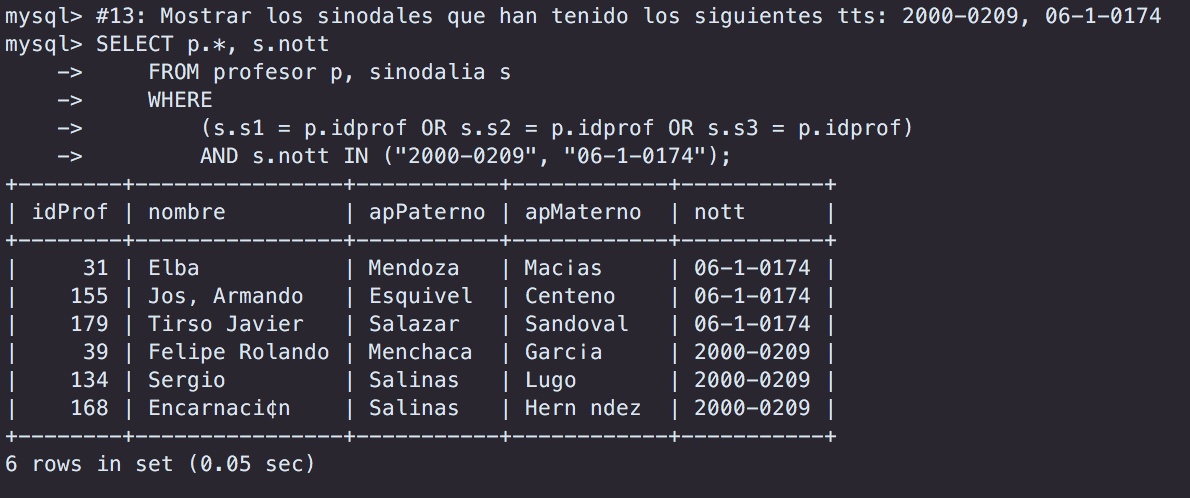
\includegraphics[width=0.45\textwidth]{BD4Reporte13}
            \caption{Mostrar los sinodales que han tenido los siguientes tts: 2000-0209, 06-1-0174}
        \end{figure}

        \begin{figure}[ht!]
            \centering
            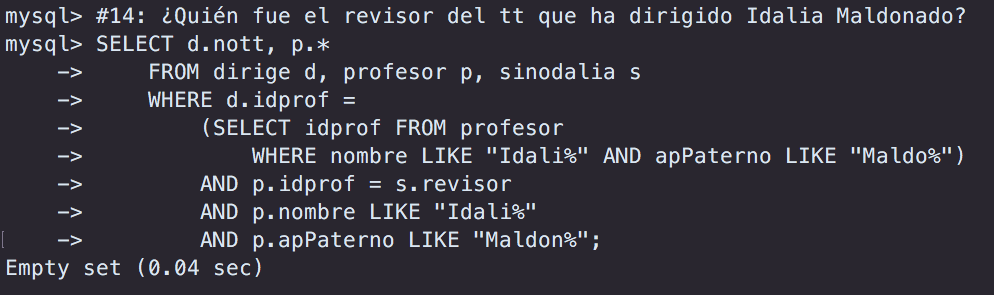
\includegraphics[width=0.45\textwidth]{BD4Reporte14}
            \caption{¿Quién fue el revisor del tt que ha dirigido Idalia Maldonado?}
        \end{figure}






% ===============================================================================
% ===================           CONCLUSIONES               ======================
% ===============================================================================
\clearpage
\section{Conclusiones}

    Gracias a esta practica pudimos comprender mucho mejor como es que funcionan las bases de datos
    y lo facil que puede llegar a ser obtener justo la información que necesitamos para su uso en los
    en sistemas computacionales.

    Vimos lo poderoso que puede llegar a ser SQL y como podemos modificar nuestros querys para obtener
    justo las tuplas que necesitamos, ordenarlas a nuestro antojo incluso (usando like y comodines)
    sin saber escepecificamente como esta escrita nuestra información.




% =====================================================
% ============        BIBLIOGRAPHY   ==================
% =====================================================
\bibliographystyle{plain}
\begin{thebibliography}{9}

    % ============ REFERENCE #1 ========
    \bibitem{Libro} 
        \texttt{Databases, Liberty Hall Chichester 1999}
        Bob Hudson

    \bibitem{Libro2} 
        \texttt{Computer Science Distilled,}


     

\end{thebibliography}



\end{document}